% Select T1 before IEEEtran initializes Times, including with XeTeX/Tectonic.
\RequirePackage[T1]{fontenc}
\documentclass[journal]{IEEEtran}

% GRSL submission manuscript: IEEE journal format, 10 pt, two columns.
\usepackage{amsmath,amssymb,bm}
\usepackage{booktabs}
\usepackage{tabularx}
\usepackage{array}
\usepackage{graphicx}
% Enable bottom placement of double-column floats without changing spacing.
\usepackage{stfloats}
\usepackage{cite}
\usepackage{url}
\usepackage{needspace}

\newcommand{\vect}[1]{\bm{#1}}

% Original comparison images, placed without resampling; labels remain 8 pt.
\newcommand{\comparisonpanel}[3]{%
  \begin{minipage}[t]{0.24\columnwidth}
    \centering
    \includegraphics[width=\linewidth]{#1}\par
    \vspace{2pt}%
    {\footnotesize\strut #2\par\strut #3\par}
  \end{minipage}%
}

% Revision master: mark substantive reviewer responses against revision_baseline/.
% Green marks passages condensed to accommodate the revision within five pages.
% Clean mode prints normal text; Marked enables blue revisions and green condensation.
\ifdefined\GRSLMarkedRevision
  \usepackage{xcolor}
  \definecolor{RevisionBlue}{RGB}{0,76,170}
  \definecolor{CondensedGreen}{RGB}{0,112,60}
  \newcommand{\rev}[1]{{\color{RevisionBlue}#1}}
  \newcommand{\condensed}[1]{{\color{CondensedGreen}#1}}
  \makeatletter
  \def\ps@grslrevision{%
    \def\@oddhead{{\normalfont\scriptsize%
      \textcolor{RevisionBlue}{Blue: revisions addressing reviewer comments.}\quad
      \textcolor{CondensedGreen}{Green: condensed passages.}}%
      \hfil{\normalfont\small\thepage}}%
    \let\@evenhead\@oddhead
    \def\@oddfoot{}\let\@evenfoot\@oddfoot}
  \let\ps@IEEEtitlepagestyle\ps@grslrevision
  \pagestyle{grslrevision}
  \makeatother
\else
  \newcommand{\rev}[1]{#1}
  \newcommand{\condensed}[1]{#1}
\fi

\begin{document}

\title{SAR Despeckling via Fourier Refinement and
Representation-Consistent Reconstruction}

\author{Hongyu~Chen, Peng~Liu,~\IEEEmembership{Senior~Member,~IEEE}%
\thanks{\raggedright\emph{(Corresponding author: Peng Liu.)}\par
The authors are with the Key Laboratory of Information Science of Electromagnetic Waves, Fudan University, Shanghai, China (e-mail: \mbox{pliu@fudan.edu.cn}).}}

\maketitle

\begin{abstract}
\condensed{We extend Trans-SAR with six Fourier refinement blocks, log inversion before intensity compensation, and encoder-frozen masked adaptation for real synthetic aperture radar (SAR). On 8,400 simulated pairs from 21 UCMerced classes and four look numbers, one blind model achieves macro-averaged peak signal-to-noise ratio (PSNR) and structural similarity index (SSIM) of 28.14~dB and 0.7791, leading PSNR at every look. Removing Fourier refinement reduces PSNR by 1.68~dB. \rev{On 20 external ICEYE scenes, adaptation lowers mean M-index from 2.4582 to 1.4634 and raises the edge-preservation index from 0.5948 to 0.8218.}}
\end{abstract}

\begin{IEEEkeywords}
Despeckling, Fourier refinement, self-supervised adaptation, synthetic aperture radar, Transformer.
\end{IEEEkeywords}

\section{Introduction}
\condensed{SAR speckle obscures edges, texture, and bright scatterers, while clean references are scarce~\cite{fracastoro2021overview}. Unit-mean Gamma models support controlled multilook tests; spatial correlation and processing artifacts complicate transfer to focused observations.}

Lee filtering uses local statistics~\cite{lee1980}; SAR-BM3D uses nonlocal recurrence and transform-domain shrinkage~\cite{parrilli2012}. Supervised CNNs learn paired priors~\cite{chierchia2017}, and SAR-CAM adds continuous multiscale attention~\cite{ko2022}. Trans-SAR couples a hierarchical Transformer encoder with convolutional reconstruction~\cite{perera2022}; later models add dynamic gates and noise-guided multiscale fusion~\cite{shen2025,zhang2025}. SAR-FDD and DATNet use frequency decomposition alongside spatial processing~\cite{shen2025,zhao2024}, while transformed conditional diffusion addresses multiplicative statistics~\cite{ma2024}. Spectral overlap between speckle and scene structure motivates joint local and full-spectrum refinement without predefined bands.

\condensed{For real observations, SAR2SAR uses multitemporal acquisitions~\cite{dalsasso2021}; Speckle2Void combines blind-spot likelihood training and decorrelation~\cite{molini2022}; Speckle2Self uses masked self-supervision with attention~\cite{lin2025}. SDS-SAR forms intensity-only pairs by correlation-aware sampling~\cite{chen2026}, whereas SDUDNet uses unpaired clean and noisy images~\cite{bo2025}.}

\condensed{We add six Fourier-domain refinement (FDR) blocks, exact log inversion before intensity compensation, and encoder-frozen masked post-adaptation (AMS) to Trans-SAR (Fig.~\ref{fig:overview}). \rev{Ablations cover four look numbers; external testing uses 20 ICEYE acquisitions.}}

% Scope retained: explicit Trans-SAR inheritance; actual six-block layout;
% exact inverse only applies to the bounded log transform; no look-number input;
% parent-disjoint real evaluation; no clean-target or unbiasedness claim.
% All 15 literature keys cited by the original Introduction/Related Work remain.

\begin{figure*}[!t]
  \centering
  \includegraphics[width=0.86\textwidth]{figures/fig1_overall_architecture.pdf}
  \caption{\condensed{(a) Architecture: gray denotes inherited operators; colors mark additions. Tensor labels show spatial size and channels. (b) Decoder skips and guidance modulation (GM). (c) Intensity reconstruction after log inversion.}}
  \label{fig:overview}
\end{figure*}

\section{Proposed Method}
\subsection{Observation and Reconstruction Path}
Let \(\vect{X},\vect{Y}\in[0,1]^{H\times W}\) denote a clean intensity proxy and its noisy observation. Synthetic pairs use independent Gamma speckle~\cite{perera2022} with look number \(L\). We clip the simulated intensities to \([0,1]\):
\begin{equation}
\begin{aligned}
\vect{Y} &= \operatorname{clip}(\vect{X}\odot\vect{N},0,1),\\
N_{ij} &\sim \operatorname{Gamma}(L,L^{-1}).
\end{aligned}
\label{eq:observation}
\end{equation}
\condensed{Speckle has unit mean and variance \(L^{-1}\) before clipping. The normalized logarithmic mapping and its exact inverse are}
\begin{equation}
T_{\alpha}(\vect{Y})=
\frac{\log(1+\alpha\vect{Y})}{\log(1+\alpha)},
\label{eq:log}
\end{equation}
\begin{equation}
T_{\alpha}^{-1}(\widehat{\vect{Z}})=
\frac{\exp[\widehat{\vect{Z}}\log(1+\alpha)]-1}{\alpha}.
\label{eq:inverse}
\end{equation}
\condensed{The mapping moderates bright intensities.}

Trans-SAR supplies overlap embeddings, spatial-reduction attention, and basic upsampling~\cite{perera2022}. Its five encoder stages have widths (32, 64, 128, 320, 512), head counts (1, 1, 2, 4, 8), depths (3, 3, 4, 6, 3), and resolutions from \(128^2\) to \(8^2\). After bottleneck refinement, five decoder stages apply upsampling, available skip fusion, FDR, residual convolution, and guidance modulation in that order. A sigmoid head predicts bounded log intensity for inversion before intensity compensation.

\subsection{Fourier Refinement and Guided Compensation}
For feature \(\vect{F}\), FDR runs a spatial branch (depthwise \(3\times3\), pointwise projection, and Gaussian error linear unit (GELU)) alongside an orthonormal two-dimensional real fast Fourier transform (FFT):
\begin{equation}
\begin{aligned}
\vect{Q} &= \operatorname{rFFT2}(\vect{F}),\\
\vect{Q}_{c} &= [\operatorname{Re}(\vect{Q}),
                   \operatorname{Im}(\vect{Q})].
\end{aligned}
\label{eq:fft}
\end{equation}
\condensed{Following~\cite{chi2020ffc}, two real-valued \(1\times1\) convolutions with GELU mix real--imaginary channels, sharing weights across frequencies without convolving neighboring frequencies. Inverse real FFT produces \(\vect{F}_f\), fused with spatial feature \(\vect{F}_s\):}
\begin{equation}
\begin{aligned}
\vect{U} &= \operatorname{GELU}
 \bigl(\vect{W}_{o,1} * [\vect{F}_{s},\vect{F}_{f}]\bigr),\\
\operatorname{FDR}(\vect{F})
 &= \vect{F}+\vect{W}_{o,2}*\vect{U}.
\end{aligned}
\label{eq:fdr}
\end{equation}
\condensed{The fusion convolutions \(\vect{W}_{o,1},\vect{W}_{o,2}\) use \(1\times1,3\times3\) kernels. Six independent full-spectrum FDR blocks span the bottleneck and decoder resolutions \(16^2\)--\(256^2\), without explicit bands or complex convolution. The bottleneck projects the sum of FDR and local features, then adds it to the input with learnable scale initialized to 0.1.}

\condensed{A shared branch learns single-channel guidance from the log input without noise-map or look supervision. At each decoder scale, resized guidance and features are concatenated; pointwise and \(3\times3\) convolutions generate \(\tanh\) modulation with learnable scale initialized to 0.1. For sigmoid output \(\widehat{\vect{Z}}\), intensity compensation follows \(\widetilde{\vect{X}}=T_\alpha^{-1}(\widehat{\vect{Z}})\):}
\begin{equation}
\begin{aligned}
\vect{R}_{c} &= F_{\mathrm{comp}}
 ([\vect{Y},\widetilde{\vect{X}}]),\\
\widehat{\vect{X}} &= \operatorname{clip}
 (\widetilde{\vect{X}}+\gamma_c\vect{R}_{c},0,1).
\end{aligned}
\label{eq:compensation}
\end{equation}
\condensed{The compensator uses two \(3\times3\), 32-channel GELU layers and a single-channel residual head, with learnable \(\gamma_c\) initialized to 0.1. Both summands are intensities; final clipping bounds the output.}

\Needspace{7\baselineskip}
\subsection{Supervision and Masked Adaptation}
\condensed{Supervised learning combines mean squared error and total variation (TV)~\cite{perera2022}:}
\begin{equation}
\mathcal{L}_{\mathrm{sup}}=
\frac{1}{HW}\lVert\widehat{\vect{X}}-\vect{X}\rVert_2^2
+\lambda_{\mathrm{TV}}^{\mathrm{sup}}\operatorname{TV}(\widehat{\vect{X}}).
\label{eq:supervised}
\end{equation}
TV is the sum of the mean absolute horizontal and vertical neighbor differences. \rev{The TV weights balance data fidelity and spatial smoothness and are selected separately on the corresponding validation splits (Section~III-B).} Following masked self-supervision~\cite{lin2025}, our AMS implementation masks pixels independently with probability 0.2 and uses their original noisy values as targets for masked L1 loss with TV on the full prediction:
\begin{equation}
\begin{gathered}
\vect{Y}_m=\vect{Y}\odot(1-\vect{M}),\qquad
\widehat{\vect{X}}_m=f_{\theta}(\vect{Y}_m),\\[3pt]
\mathcal{L}_{\mathrm{AMS}}=
\frac{\lVert\vect{M}\odot(\widehat{\vect{X}}_m-\vect{Y})\rVert_1}
{\max(\lVert\vect{M}\rVert_1,1)}
+\lambda_{\mathrm{AMS}}\operatorname{TV}(\widehat{\vect{X}}_m).
\end{gathered}
\label{eq:ams}
\end{equation}
\condensed{Mask ones identify masked pixels; outputs are intensities. With only the Transformer encoder frozen, the bottleneck, decoder, guidance, head, and compensator adapt for eight epochs at \rev{\(2\times10^{-6}\)}. Training masks are resampled and validation masks fixed. AMS supplies \(\vect{Y}_m\) throughout the network, including compensation; inference uses unmasked observations.}

\begin{table*}[!b]
\caption{UCM-21 Gamma-Speckle Results on 8,400 Fixed Pairs}
\label{tab:main}
\centering
\footnotesize
\setlength{\tabcolsep}{3.2pt}
\renewcommand{\arraystretch}{1.08}
\begin{tabular*}{0.86\textwidth}{@{\extracolsep{\fill}}llccccc@{}}
\toprule
\textbf{Method} & \textbf{Look mode} &
\shortstack{\(L=1\)\\PSNR / SSIM} &
\shortstack{\(L=2\)\\PSNR / SSIM} &
\shortstack{\(L=4\)\\PSNR / SSIM} &
\shortstack{\(L=8\)\\PSNR / SSIM} &
\shortstack{Macro\\PSNR / SSIM} \\
\midrule
Noisy       & --                & 12.95 / 0.2069 & 14.98 / 0.2870 & 17.37 / 0.3840 & 20.01 / 0.4916 & 16.33 / 0.3424 \\
Lee-MMSE    & oracle-\(L\)      & 21.23 / 0.5212 & 23.05 / 0.5999 & 24.71 / 0.6757 & 26.33 / 0.7455 & 23.83 / 0.6356 \\
SAR-BM3D    & oracle-\(L\)      & 25.24 / \textbf{0.7234} & 26.78 / \underline{0.7612} & \underline{28.14} / \textbf{0.7967} & 29.77 / \underline{0.8243} & 27.48 / \underline{0.7764} \\
SAR-CAM     & blind             & 22.68 / 0.5622 & 23.54 / 0.6138 & 25.89 / 0.7295 & 28.10 / 0.7949 & 25.05 / 0.6751 \\
Trans-SAR   & blind             & \underline{25.53} / 0.6446 & \underline{27.22} / 0.6963 & 28.12 / 0.7397 & \underline{29.78} / 0.7336 & \underline{27.66} / 0.7036 \\
\textbf{Ours (Full)} & blind    & \textbf{25.93} / \underline{0.7169} & \textbf{27.94} / \textbf{0.7930} & \textbf{28.57} / \underline{0.7754} & \textbf{30.13} / \textbf{0.8312} & \textbf{28.14} / \textbf{0.7791} \\
\midrule
\rev{\(p\) (vs Trans-SAR)} & -- & -- & -- & -- & -- & \rev{0.007 / 0.003} \\
\rev{\(p\) (vs SAR-BM3D)} & -- & -- & -- & -- & -- & \rev{0.011 / 0.002} \\
\bottomrule
\end{tabular*}
\vspace{1pt}
\parbox{0.86\textwidth}{\footnotesize PSNR is in dB. Best and second-best values among despeckling methods are bold and underlined, respectively. Oracle-\(L\) methods receive the nominal look number; blind methods do not. \rev{\(p\): Holm-adjusted paired tests versus Ours (Full), for macro PSNR / SSIM.}}
\end{table*}

\section{Experiments}
\subsection{Datasets and Evaluation Protocol}
\condensed{NWPU-RESISC45~\cite{cheng2017} supplies 900 training and 225 validation images (20/5 per class), using squared grayscale values as clean intensity proxies. \rev{Approximately 50,000} training presentations balance \(L\in\{1,2,4,8\}\) deterministically, with paired flips and right-angle rotations. Four fixed realizations per validation source yield 900 pairs.}

\condensed{The 2,100 UCMerced images from 21 classes~\cite{yang2010} are held out from model selection and yield 8,400 fixed test pairs, one corruption per source and look. Images are bilinearly resized to \(256\times256\), if needed, before applying~\eqref{eq:observation} once. This evaluates transfer between optical collections under simulated speckle.}

\rev{Mendeley dataset fs455tz88y, version~1~\cite{vasquez2024data}, supplies 1,175 adaptation-training and 146 validation parents (4,700/584 patches). Each parent's four patches stay together. External testing replaces the earlier 148-parent internal evaluation with 20 complete ICEYE Open Data acquisitions~\cite{iceyeOpenData}, excluded from training, validation, and model selection.}

\rev{The selected NWPU checkpoint initializes real-SAR adaptation. After each epoch, minimum validation intensity MSE selects supervision and minimum masked loss selects AMS. We fix weights and hyperparameters before synthetic and real-SAR testing.}

\rev{For the 20-scene quantitative evaluation, methods share native SLC grids and decoded linear intensity. Inference normalization is inverted and contextual tiles are assembled before whole-scene measurement. Display stretching is excluded, and the 20 parent scenes receive equal weight.}

\rev{Two-sided paired \(t\)-tests use Holm correction across 15 comparisons (\(p<0.05\)). Pairing uses 2,100 source images after averaging four looks, or 20 independent real-SAR parents. Real-SAR variability uses sample SD; the mean M-index reduction has an unadjusted 95\% \(t\) confidence interval (CI) from 20 paired differences (19 degrees of freedom).}

\subsection{Implementation, Baselines, and Metrics}
\condensed{We use Adam for \rev{50 epochs (approximately 50,000 updates)}, with batch size 1, initial rate \rev{\(2\times10^{-4}\)}, and weight decay \(10^{-5}\). Validation plateaus halve the rate, down to \(10^{-6}\). Synthetic validation selects \(\alpha=10\) from \(\{1,5,10,20,50\}\) by PSNR, supported by SSIM. \rev{Table~\ref{tab:lambda} selects \(\lambda_{\mathrm{TV}}^{\mathrm{sup}}=0.03\) by macro PSNR/SSIM (0.05 is similar) and \(\lambda_{\mathrm{AMS}}=10^{-3}\) by M-index; larger AMS weights worsen M-index/EPI. Both remain fixed for testing.} One pre-adaptation checkpoint (Full/Ours-base) handles all looks. NWPU validation selects Lee-MMSE's window; SAR-BM3D takes square-root input and squares its output. Both receive nominal \(L\) (oracle-\(L\)); SAR-CAM~\cite{ko2022}, Trans-SAR~\cite{perera2022}, and ours receive only corrupted intensity.}

\rev{Training and validation losses decrease overall (Figs.~\ref{fig:learning_supervised} and~\ref{fig:learning_ams}); supervised validation fluctuates. Stars mark validation minima at supervised epoch 47 and AMS epoch 8.}

% R2.2: the author confirmed these loss records and learning rates on 2026-11-13.
% Source: ExperimentalRecord.txt, lines 251-300 (supervision), 310-317 (AMS).
\begin{figure}[!t]
  \centering
  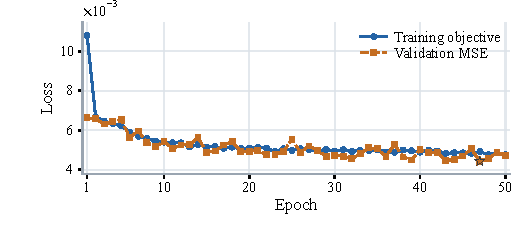
\includegraphics[width=\columnwidth]{figures/fig_learning_supervised.pdf}
  \caption{\rev{Training and validation losses during supervised learning.}}
  \label{fig:learning_supervised}
\end{figure}

\begin{figure}[!t]
  \centering
  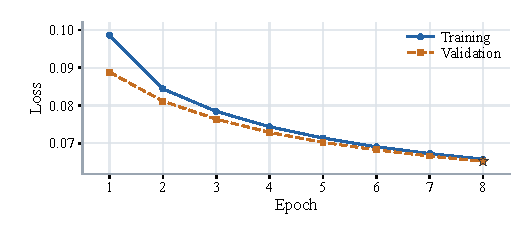
\includegraphics[width=\columnwidth]{figures/fig_learning_ams.pdf}
  \caption{\rev{Training and validation losses during AMS adaptation.}}
  \label{fig:learning_ams}
\end{figure}

% R2.1: author-supplied results from the independent validation splits.
% The two groups are separate sweeps; rows are not joint configurations.
\begin{table}[!t]
\caption{\rev{Validation Sensitivity to the TV Weights}}
\label{tab:lambda}
\centering
\footnotesize
\setlength{\tabcolsep}{2.5pt}
\renewcommand{\arraystretch}{1.05}
\rev{\begin{tabular*}{\columnwidth}{@{\extracolsep{\fill}}cccccc@{}}
\toprule
\multicolumn{3}{c}{NWPU validation} & \multicolumn{3}{c}{Real-SAR validation} \\
\cmidrule(lr){1-3}\cmidrule(lr){4-6}
\(\lambda_{\mathrm{TV}}^{\mathrm{sup}}\) & PSNR\,$\uparrow$ & SSIM\,$\uparrow$ & \(\lambda_{\mathrm{AMS}}\) & M-index\,$\downarrow$ & EPI \\
\midrule
0.01 & 28.02 & 0.7728 & \(10^{-5}\) & 1.5824 & 0.8436 \\
\textbf{0.03} & 28.20 & 0.7814 & \(10^{-4}\) & 1.5107 & 0.8221 \\
0.05 & 28.17 & 0.7806 & \(\mathbf{10^{-3}}\) & 1.4618 & 0.7965 \\
0.08 & 28.08 & 0.7773 & \(10^{-2}\) & 1.5362 & 0.6512 \\
0.10 & 27.99 & 0.7731 & \(10^{-1}\) & 1.8074 & 0.4238 \\
\bottomrule
\end{tabular*}}
\vspace{1pt}
\parbox{\columnwidth}{\footnotesize\rev{PSNR is in dB. Bold weights are selected in separate sweeps.}}
\end{table}

\rev{PSNR/SSIM average equally across UCM-21 classes and looks. ENL, \(\mu^2/\sigma^2\) with population variance, averages ten fixed \(64\times64\) input ROIs per scene or five \(32\times32\) sub-ROIs per Table~\ref{tab:real_scenes} region. It measures local smoothness and is not ranked.}

\rev{For ratio \(R=Y/\widehat X\), M-index~\cite{gomez2017} combines half the average unit-mean and relative-ENL deviations in qualifying windows with \(100|h_R-\bar h_{\pi(R)}|/h_R\): \(h\) is GLCM homogeneity and \(\pi\) permutes pixels. We use \(25\times25\) windows, 0.03 tolerance, eight gray levels, and 100 permutations; lower is better. EPI~\cite{ma2024epi} is \(\sum|\Delta_d\widehat X|/\sum|\Delta_dY|\), where \(\Delta_d\) is the lower-right diagonal difference. Residual speckle and global gain can increase EPI~\cite{vasquez2025ratio}.}

\rev{RGPI~\cite{ma2022rgpi} averages \(W_i\log f(Q_{id}\mid q_{id})\) over valid pixels and four directions. \(Q,q\) are ratios of opposite \(3\times3\) neighborhood means in input/output; nonnegative Lee weights \(W_i\) use \(7\times7\) input windows. For \(a=9L\), \(L=1\),
\begin{equation}
f(Q\mid q)=\frac{\Gamma(2a)}{\Gamma(a)^2}\frac{q^aQ^{a-1}}{(Q+q)^{2a}}.
\label{eq:rgpi}
\end{equation}
Higher RGPI indicates ratio-gradient retention on fixed input support. It is invariant to positive global gain; Noisy attains its upper bound and is excluded from ranking.}

\subsection{Synthetic Comparison}
\condensed{Table~\ref{tab:main}: ours leads PSNR at every look and macro PSNR/SSIM (28.14~dB/0.7791), exceeding Trans-SAR by 0.48~dB/0.0755 and SAR-BM3D by 0.66~dB/0.0027. \rev{Both macro gains are significant against each baseline (adjusted \(p\leq0.011\)).} Ours leads SSIM at \(L=2,8\); SAR-BM3D at \(L=1,4\).}

\condensed{In Fig.~\ref{fig:synthetic_qual}, ours retains roof contours that LEE blurs. Building outlines in our ratio image indicate residual structural content.}

\begin{figure}[!t]
  \centering
  \begin{tabular}{@{}c@{\hspace{0.01\columnwidth}}c@{\hspace{0.01\columnwidth}}c@{\hspace{0.01\columnwidth}}c@{}}
    \comparisonpanel{figures/fig4/00_Clean.png}{(a)}{Clean} &
    \comparisonpanel{figures/fig4/01_Noisy.png}{(b)}{Noisy} &
    \comparisonpanel{figures/fig4/LEE-MMSE.png}{(c)}{LEE} &
    \comparisonpanel{figures/fig4/SAR-BM3D.png}{(d)}{SAR-BM3D} \\[3pt]
    \comparisonpanel{figures/fig4/SAR-CAM.png}{(e)}{SAR-CAM} &
    \comparisonpanel{figures/fig4/SAR-Trans.png}{(f)}{Trans-SAR} &
    \comparisonpanel{figures/fig4/Ours-base.png}{(g)}{Ours} &
    \comparisonpanel{figures/fig4/Ours-base_ratio.png}{(h)}{Ours ratio}
  \end{tabular}
  \caption{\condensed{UCMerced buildings comparison, with a shared field of view and original grayscale rendering. LEE denotes Lee-MMSE; (h) is the Ours ratio image.}}
  \label{fig:synthetic_qual}
\end{figure}

\subsection{Generalization across Three UCMerced Scene Types}
\condensed{Table~\ref{tab:ucm_scenes} evaluates 100 held-out samples each of agriculture, buildings, and dense residential scenes at \(L=4\), covering smooth areas, regular boundaries, and dense texture.}

\begin{table}[!t]
\caption{Generalization on Three UCMerced Scene Types at \(L=4\)}
\label{tab:ucm_scenes}
\centering
\footnotesize
\setlength{\tabcolsep}{3.0pt}
\renewcommand{\arraystretch}{1.08}
\begin{tabular*}{\columnwidth}{@{\extracolsep{\fill}}lccc@{}}
\toprule
\textbf{Scene} & \textbf{Num.} &
\shortstack{\textbf{Noisy}\\PSNR / SSIM} &
\shortstack{\textbf{Ours-base}\\PSNR / SSIM} \\
\midrule
Agricultural & 100 & \rev{17.76} / 0.4218 & \textbf{\rev{29.15} / 0.7446} \\
Buildings    & 100 & \rev{16.66} / 0.4625 & \textbf{\rev{27.68} / 0.7883} \\
Dense residential & 100 & \rev{17.55} / 0.4557 & \textbf{\rev{30.44} / 0.7941} \\
\midrule
Average      & 300 & \rev{17.32} / 0.4467 & \textbf{\rev{29.09} / 0.7757} \\
\bottomrule
\end{tabular*}
\vspace{1pt}
\parbox{\columnwidth}{\footnotesize \condensed{PSNR: dB. Average: three equal-sized groups. Ours-base: before adaptation. Bold: improvement over Noisy.}}
\end{table}

\condensed{PSNR/SSIM gains are 11.02--12.89~dB/0.3228--0.3384, with the highest restored scores in dense residential scenes.}

\subsection{Ablation Study}
\condensed{Table~\ref{tab:ablation} compares representation, compensation, and FDR.}

\begin{table}[!t]
\caption{\rev{Ablation and Model Complexity on UCM-21}}
\label{tab:ablation}
\centering
\footnotesize
\setlength{\tabcolsep}{2.7pt}
\renewcommand{\arraystretch}{1.08}
\begin{tabular*}{\columnwidth}{@{\extracolsep{\fill}}lrrrr@{}}
\toprule
\textbf{Variant} & \textbf{PSNR} & \textbf{SSIM} &
\rev{\shortstack{\textbf{Params}\\(M)}} &
\rev{\shortstack{\textbf{FLOPs}\\(G)}} \\
\midrule
Intensity-only & \rev{23.68} & 0.6871 & \rev{39.343} & \rev{26.60} \\
Log-only & \rev{22.22} & 0.7121 & \rev{39.343} & \rev{26.60} \\
Full w/o all FDR & \rev{26.46} & 0.7612 & \rev{31.608} & \rev{23.97} \\
\rev{Full w/o bottleneck FDR} & \underline{\rev{27.13}} & \underline{\rev{0.7704}} & \rev{34.101} & \rev{27.38} \\
\rev{Full w/o decoder FDR} & \rev{26.67} & \rev{0.7679} & \rev{36.860} & \rev{24.55} \\
\textbf{Full} & \textbf{\rev{28.14}} & \textbf{0.7791} & \rev{39.353} & \rev{27.95} \\
\midrule
\rev{\(p\) (vs Log-only)} & \rev{0.006} & \rev{0.006} & -- & -- \\
\rev{\(p\) (vs w/o all FDR)} & \rev{0.014} & \rev{0.001} & -- & -- \\
\rev{\(p\) (vs w/o bottleneck FDR)} & \rev{0.009} & \rev{0.002} & -- & -- \\
\rev{\(p\) (vs w/o decoder FDR)} & \rev{0.003} & \rev{0.007} & -- & -- \\
\bottomrule
\end{tabular*}
\vspace{1pt}
\parbox{\columnwidth}{\footnotesize PSNR is in dB. Intensity-only omits the log mapping and compensation; Log-only retains the log/inverse mapping without compensation. \rev{FLOPs use a \(1\times1\times256\times256\) input. \(p\): Holm-adjusted paired tests versus Full.}}
\end{table}

\condensed{\rev{FDR ablations retain the log/inverse mapping, compensator, and local bottleneck branch. Removing bottleneck/decoder FDR reduces PSNR by 1.01/1.47~dB;} removing all FDR reduces PSNR/SSIM by 1.68~dB/0.0179.}

\condensed{Full gains \rev{5.92~dB}/0.0670 over Log-only, supporting compensation with FDR. \rev{Both metrics improve over all four tested variants (adjusted \(p\leq0.014\)).} Log-only lowers PSNR but raises SSIM versus Intensity-only.}

\subsection{Real-SAR Adaptation}
\rev{Table~\ref{tab:real} compares four baselines and matched Ours-base/Ours+AMS on 20 complete ICEYE scenes. Apart from fixed-ROI ENL, metrics use the full valid image support.}

\begin{table}[!t]
\caption{\rev{No-Reference Results on 20 Complete ICEYE Scenes}}
\label{tab:real}
\centering
\footnotesize
\setlength{\tabcolsep}{1.1pt}
\renewcommand{\arraystretch}{1.04}
\rev{\begin{tabular*}{\columnwidth}{@{\extracolsep{\fill}}lrrrr@{}}
\toprule
\textbf{Method} & \textbf{ENL} & \textbf{M-index}\,$\downarrow$ & \textbf{EPI} & \textbf{RGPI}\,$\uparrow$ \\
\midrule
Noisy & 14.37 & -- & \(1.000{\pm}0.000\) & \(0.897{\pm}0.030\) \\
SAR-BM3D & 29.33 & \(1.746{\pm}0.143\) & \(\underline{0.808}{\pm}0.102\) & \(0.281{\pm}0.021\) \\
SAR2SAR & 11.64 & \(3.453{\pm}0.133\) & \(0.593{\pm}0.021\) & \(\underline{0.706}{\pm}0.028\) \\
SDUDNet & 14.89 & \(\underline{1.657}{\pm}0.053\) & \(0.403{\pm}0.033\) & \(0.680{\pm}0.018\) \\
Trans-SAR & 127.21 & \(2.675{\pm}0.098\) & \(0.255{\pm}0.013\) & \(0.166{\pm}0.038\) \\
Ours-base & 151.77 & \(2.458{\pm}0.069\) & \(0.595{\pm}0.072\) & \(0.548{\pm}0.107\) \\
Ours+AMS & 36.81 & \(\mathbf{1.463}{\pm}0.083\) & \(\mathbf{0.822}{\pm}0.053\) & \(\mathbf{0.753}{\pm}0.062\) \\
\midrule
\(p\) (AMS/base) & -- & \(<0.001\) & \(<0.001\) & \(<0.001\) \\
\bottomrule
\end{tabular*}}
\vspace{1pt}
\parbox{\columnwidth}{\footnotesize\rev{M-index, EPI, RGPI: mean \(\pm\) sample SD across 20 parents; ENL: mean. Noisy is excluded from ranking; its M-index is undefined. Bold/underlined means rank first/second. \(p\): Holm-adjusted paired tests, AMS versus base.}}
\end{table}

\rev{AMS leads mean M-index, EPI, and RGPI among filtered outputs. M-index falls from \(2.458\pm0.069\) to \(1.463\pm0.083\), a mean reduction of 0.9948 (95\% CI: [0.9657, 1.0239]), or 40.47\%. EPI rises from \(0.595\pm0.072\) to \(0.822\pm0.053\), and RGPI from \(0.548\pm0.107\) to \(0.753\pm0.062\) (mean \(\pm\) SD). All three paired improvements are significant (adjusted \(p<0.001\)); ENL decreases.}

\rev{Fig.~\ref{fig:real_qual} compares the Paris Le Bourget GRD crop (October 28, 2025). Ours-base (f) broadens bright structures. Ours+AMS (g) reduces fluctuations in H and retains sharper boundaries and scatterers in S/T. Its ratio (h) shows granular residuals with faint scene contours.}

\begin{figure}[!t]
  \centering
  \begin{tabular}{@{}c@{\hspace{0.01\columnwidth}}c@{\hspace{0.01\columnwidth}}c@{\hspace{0.01\columnwidth}}c@{}}
    \comparisonpanel{figures/fig5_paris/a_noisy.png}{(a)}{Noisy} &
    \comparisonpanel{figures/fig5_paris/b_sar-bm3d.png}{(b)}{SAR-BM3D} &
    \comparisonpanel{figures/fig5_paris/c_sar2sar.png}{(c)}{SAR2SAR} &
    \comparisonpanel{figures/fig5_paris/d_sdudnet.png}{(d)}{SDUDNet*} \\[3pt]
    \comparisonpanel{figures/fig5_paris/e_trans-sar.png}{(e)}{Trans-SAR} &
    \comparisonpanel{figures/fig5_paris/f_ours-bas.png}{(f)}{Ours-base} &
    \comparisonpanel{figures/fig5_paris/g_ours-ams.png}{(g)}{Ours+AMS} &
    \comparisonpanel{figures/fig5_paris/h_ours-ams-ratio.png}{(h)}{Ours+AMS ratio}
  \end{tabular}
  \caption{\rev{ICEYE Paris GRD, $3072\times3072$ crop. H/S/T mark $384\times384$ homogeneous, structural, and textured regions. (a)--(g): intensity, $-18$ to $0$~dB; (h): $10\log_{10}(Y/\widehat X)$, $-5$ to $5$~dB. *SDUDNet uses display-domain input.}}
  \label{fig:real_qual}
\end{figure}

\subsection{Scene-Wise No-Reference Evaluation on Real SAR}
\rev{Each of 20 parents contributes three nonoverlapping \(256\times256\) regions: homogeneous (H), structural (S), and textured (T). Input-only screening selects low variation, coherent boundaries, and distributed texture, with coordinates fixed by noisy-input review. Regions are extracted from full predictions. Average first averages H/S/T within each parent, then summarizes the 20 parent averages.}

% Source: author-updated Desktop/实验结果.md, 2026-11-15.
% Mean and SD: latest author-updated GRSL_统计补充待填表.md, 2026-11-16.
\begin{table}[!t]
\caption{\rev{No-Reference Results by ICEYE Region Type}}
\label{tab:real_scenes}
\centering
\footnotesize
\setlength{\tabcolsep}{1.1pt}
\renewcommand{\arraystretch}{1.04}
\rev{\begin{tabular*}{\columnwidth}{@{\extracolsep{\fill}}lrrrr@{}}
\toprule
\textbf{Method} & \textbf{ENL} & \textbf{M-index}\,$\downarrow$ & \textbf{EPI} & \textbf{RGPI}\,$\uparrow$ \\
\midrule
\multicolumn{5}{@{}l@{}}{\textit{Homogeneous: 20 regions}} \\
Noisy & 28.23 & -- & \(1.000{\pm}0.000\) & \(0.287{\pm}0.039\) \\
Ours-base & 213.34 & \(6.342{\pm}0.639\) & \(0.535{\pm}0.078\) & \(0.120{\pm}0.012\) \\
Ours+AMS & 46.23 & \(\mathbf{3.452}{\pm}0.413\) & \(\mathbf{0.754}{\pm}0.092\) & \(\mathbf{0.167}{\pm}0.009\) \\
\midrule
\multicolumn{5}{@{}l@{}}{\textit{Structural: 20 regions}} \\
Noisy & 21.39 & -- & \(1.000{\pm}0.000\) & \(0.453{\pm}0.113\) \\
Ours-base & 189.23 & \(1.238{\pm}0.093\) & \(0.439{\pm}0.028\) & \(0.158{\pm}0.030\) \\
Ours+AMS & 39.66 & \(\mathbf{0.782}{\pm}0.027\) & \(\mathbf{0.647}{\pm}0.081\) & \(\mathbf{0.396}{\pm}0.074\) \\
\midrule
\multicolumn{5}{@{}l@{}}{\textit{Textured: 20 regions}} \\
Noisy & 13.43 & -- & \(1.000{\pm}0.000\) & \(0.653{\pm}0.102\) \\
Ours-base & 173.56 & \(0.248{\pm}0.047\) & \(0.360{\pm}0.076\) & \(0.243{\pm}0.028\) \\
Ours+AMS & 31.82 & \(\mathbf{0.064}{\pm}0.013\) & \(\mathbf{0.712}{\pm}0.082\) & \(\mathbf{0.491}{\pm}0.088\) \\
\midrule
\multicolumn{5}{@{}l@{}}{\textit{Average: 60 regions from 20 parents}} \\
Noisy & 21.02 & -- & \(1.000{\pm}0.000\) & \(0.464{\pm}0.063\) \\
Ours-base & 192.04 & \(2.609{\pm}0.194\) & \(0.445{\pm}0.021\) & \(0.173{\pm}0.013\) \\
Ours+AMS & 39.24 & \(\mathbf{1.433}{\pm}0.134\) & \(\mathbf{0.704}{\pm}0.029\) & \(\mathbf{0.352}{\pm}0.035\) \\
\bottomrule
\end{tabular*}}
\vspace{1pt}
\parbox{\columnwidth}{\footnotesize\rev{M-index, EPI, RGPI: mean \(\pm\) sample SD across 20 parents; Average first averages H/S/T within each parent. ENL: mean. Bold marks the better filtered mean.}}
\end{table}

\rev{AMS lowers mean M-index and raises mean EPI/RGPI in all categories. Average M-index falls from \(2.609\pm0.194\) to \(1.433\pm0.134\). ENL lies between Noisy and Ours-base, consistent with reduced smoothing.}

\section{Conclusion}
\condensed{FDR and intensity compensation after log inversion improve Trans-SAR macro PSNR/SSIM, supported by ablations. \rev{Encoder-frozen AMS improves M-index and EPI on 20 external ICEYE scenes and three region types, with less smoothing.}}

\begin{thebibliography}{00}

\bibitem{fracastoro2021overview}
G. Fracastoro, E. Magli, G. Poggi, G. Scarpa, D. Valsesia, and L. Verdoliva, ``Deep learning methods for synthetic aperture radar image despeckling: An overview of trends and perspectives,'' \emph{IEEE Geosci. Remote Sens. Mag.}, vol.~9, no.~2, pp.~29--51, 2021, doi: 10.1109/MGRS.2021.3070956.

\bibitem{lee1980}
J.-S. Lee, ``Digital image enhancement and noise filtering by use of local statistics,'' \emph{IEEE Trans. Pattern Anal. Mach. Intell.}, vol.~PAMI-2, no.~2, pp.~165--168, 1980, doi: 10.1109/TPAMI.1980.4766994.

\bibitem{parrilli2012}
S. Parrilli, M. Poderico, C. V. Angelino, and L. Verdoliva, ``A nonlocal SAR image denoising algorithm based on LLMMSE wavelet shrinkage,'' \emph{IEEE Trans. Geosci. Remote Sens.}, vol.~50, no.~2, pp.~606--616, 2012, doi: 10.1109/TGRS.2011.2161586.

\bibitem{chierchia2017}
G. Chierchia, D. Cozzolino, G. Poggi, and L. Verdoliva, ``SAR image despeckling through convolutional neural networks,'' in \emph{Proc. IEEE IGARSS}, 2017, pp.~5438--5441, doi: 10.1109/IGARSS.2017.8128234.

\bibitem{ko2022}
J. Ko and S. Lee, ``SAR image despeckling using continuous attention module,'' \emph{IEEE J. Sel. Topics Appl. Earth Observ. Remote Sens.}, vol.~15, pp.~3--19, 2022, doi: 10.1109/JSTARS.2021.3132027.

\bibitem{perera2022}
M. V. Perera, W. G. C. Bandara, J. M. J. Valanarasu, and V. M. Patel, ``Transformer-based SAR image despeckling,'' in \emph{Proc. IEEE IGARSS}, 2022, pp.~751--754, doi: 10.1109/IGARSS46834.2022.9884596.

\bibitem{shen2025}
Y. Shen, Y. Chen, Y. Wang, L. Ma, and X. Zhang, ``DATNet: Dynamic adaptive Transformer network for SAR image denoising,'' \emph{Remote Sens.}, vol.~17, no.~17, Art. no.~3031, 2025, doi: 10.3390/rs17173031.

\bibitem{zhang2025}
L. Zhang, L. Zheng, Y. Wen, F. Zhang, F. Bo, and Y. Cen, ``Effective SAR image despeckling using noise-guided Transformer and multi-scale feature fusion,'' \emph{Remote Sens.}, vol.~17, no.~23, Art. no.~3863, 2025, doi: 10.3390/rs17233863.

\bibitem{zhao2024}
X. Zhao, F. Ren, H. Sun, and Q. Qi, ``Synthetic aperture radar image despeckling based on a deep learning network employing frequency domain decomposition,'' \emph{Electronics}, vol.~13, no.~3, Art. no.~490, 2024, doi: 10.3390/electronics13030490.

\bibitem{ma2024}
Y. Ma, P. Ke, H. Aghababaei, L. Chang, and J. Wei, ``Despeckling SAR images with Log-Yeo--Johnson transformation and conditional diffusion models,'' \emph{IEEE Trans. Geosci. Remote Sens.}, vol.~62, Art. no.~5215417, 2024, doi: 10.1109/TGRS.2024.3419083.

\bibitem{dalsasso2021}
E. Dalsasso, L. Denis, and F. Tupin, ``SAR2SAR: A semi-supervised despeckling algorithm for SAR images,'' \emph{IEEE J. Sel. Topics Appl. Earth Observ. Remote Sens.}, vol.~14, pp.~4321--4329, 2021, doi: 10.1109/JSTARS.2021.3071864.

\bibitem{molini2022}
A. B. Molini, D. Valsesia, G. Fracastoro, and E. Magli, ``Speckle2Void: Deep self-supervised SAR despeckling with blind-spot convolutional neural networks,'' \emph{IEEE Trans. Geosci. Remote Sens.}, vol.~60, Art. no.~5204017, 2022, doi: 10.1109/TGRS.2021.3065461.

\bibitem{lin2025}
H. Lin, X. Su, Z. Zeng, C. Xing, and J. Yin, ``Speckle2Self: Learning self-supervised despeckling with attention mechanism for SAR images,'' \emph{Remote Sens.}, vol.~17, no.~23, Art. no.~3840, 2025, doi: 10.3390/rs17233840.

\bibitem{chen2026}
L. Chen, Y. Yin, H. Shi, J. He, and W. Li, ``Self-supervised despeckling based solely on SAR intensity images: A general strategy,'' \emph{ISPRS J. Photogramm. Remote Sens.}, vol.~231, pp.~854--873, 2026, doi: 10.1016/j.isprsjprs.2025.11.025.

\bibitem{bo2025}
F. Bo, X. Ma, S. Hu, G. An, Y. Li, and Y. Cen, ``Speckle-driven unsupervised despeckling for SAR images,'' \emph{IEEE J. Sel. Topics Appl. Earth Observ. Remote Sens.}, vol.~18, pp.~13023--13034, 2025, doi: 10.1109/JSTARS.2025.3568854.

\bibitem{chi2020ffc}
L. Chi, B. Jiang, and Y. Mu, ``Fast Fourier convolution,'' in \emph{Advances in Neural Information Processing Systems}, vol.~33, pp.~4479--4488, 2020.

\bibitem{cheng2017}
G. Cheng, J. Han, and X. Lu, ``Remote sensing image scene classification: Benchmark and state of the art,'' \emph{Proc. IEEE}, vol.~105, no.~10, pp.~1865--1883, 2017, doi: 10.1109/JPROC.2017.2675998.

\bibitem{yang2010}
Y. Yang and S. Newsam, ``Bag-of-visual-words and spatial extensions for land-use classification,'' in \emph{Proc. ACM SIGSPATIAL Int. Conf. Adv. Geogr. Inf. Syst.}, 2010, pp.~270--279, doi: 10.1145/1869790.1869829.

\bibitem{vasquez2024data}
R. Vasquez, A. A. Cardona-Mesa, L. G\'omez, C. M. Travieso-Gonz\'alez, A. Garavito Gonzalez, and E. V\'asquez-Cano, Jan. 24, 2024, ``Labeled dataset for despeckling SAR imagery,'' Mendeley Data, ver.~1, doi: 10.17632/fs455tz88y.1.

\bibitem{iceyeOpenData}
ICEYE, ``ICEYE Open Data,'' product documentation, accessed Nov.~15, 2026. [Online]. Available: \url{https://sar.iceye.com/6.0.6/opendata/opendata/}

\bibitem{gomez2017}
L. G\'omez, R. Ospina, and A. C. Frery, ``Unassisted quantitative evaluation of despeckling filters,'' \emph{Remote Sens.}, vol.~9, no.~4, Art. no.~389, 2017, doi: 10.3390/rs9040389.

\bibitem{ma2024epi}
X. Ma, L. Li, and G. Wang, ``Blind edge-retention indicator for assessing the quality of filtered (Pol)SAR images based on a ratio gradient operator and confidence interval estimation,'' \emph{Remote Sens.}, vol.~16, no.~11, Art. no.~1992, 2024, doi: 10.3390/rs16111992.

\bibitem{vasquez2025ratio}
R. D. V\'asquez-Salazar, W. S. Puche, A. C. Frery, and L. G\'omez, ``Quality assessment of despeckling filters based on the analysis of ratio images,'' \emph{Remote Sens.}, vol.~17, no.~24, Art. no.~4048, 2025, doi: 10.3390/rs17244048.

\bibitem{ma2022rgpi}
X. Ma, H. Hu, and P. Wu, ``A no-reference edge-preservation assessment index for SAR image filters under a Bayesian framework based on the ratio gradient,'' \emph{Remote Sens.}, vol.~14, no.~4, Art. no.~856, 2022, doi: 10.3390/rs14040856.

\end{thebibliography}

\end{document}
